\chapter{Overview of Optimal Transport}

\myminitoc

Le transport optimal permet de définir une géométrie et une distance sur l'ensemble des mesures de probabilités sur un espace.

\sect{Introduction}

\subs{Problème de Monge}

\begin{center}
	\begin{tikzpicture}[>=stealth']
		\draw[fill=brown!20] (-1, -1.8) rectangle (9, 0);
		\draw[fill=red, domain=0:2, smooth, variable=\x, fill opacity=0.9]
			plot({1.5*\x}, {\x * (27.21 + \x * (-126.6 + \x * (229.9 + \x * (-200.7
				+ \x * (84.24 - 13.61 * \x)))))}) -- (3.05, 0);
		\node[red] at (-0.2, 0.7) {$\mu$};
		\draw[fill=blue, fill opacity=0.9]
			(5, 0) -- (5.1, -1.2) -- (5.5, -1.2) -- (5.6, -1) -- (5.9, -1) --
			(6, -1.2) -- (6.4, -1.2) -- (6.5, -1) -- (6.8, -1) -- (6.9, -1.2) --
			(7.3, -1.2) -- (7.4, -1) -- (7.7, -1) -- (7.8, 0);
		\node[blue] at (8, -1.2) {$\nu$};
		\draw[ultra thick, purple] (0.4, 0) -- (0.4, 1.68);
		\draw[ultra thick, purple] (6.1, 0) -- (6.1, -1.2);
		\node[red] (x) at (0.4, -0.15) {$\bullet$};
		\node[blue] (y) at (6.1, 0.15) {$\bullet$};
		\node[below] at (x) {$x$};
		\node[above] at (y) {$y = T(x)$};
		\coordinate (y) at (6, 0.1);
		\draw[->, ultra thick, greenTikz, bend right=30]
			(x) edge node[below, black] {${\color{greenTikz}c}(x, T(x))$} (y);
	\end{tikzpicture}
\end{center}

\paragraph{Monge}
On se place dans un espace de probabilité $\Omega$. Puis on se donne $\mu$ et $\nu$, deux mesures de probabilités sur $\mathcal{P}(\Omega)$. De plus on se donne une fonction de coût $c : \Omega \times \Omega \rightarrow \R$. Cette fonction peut être la distance euclidienne par exemple. Le problème de Monge est alors le suivant :
$$ \int_{\Omega} c \left( x, T(x) \right) \mu(x) $$
\vspace{-2mm}
$$ \text{s.t.} \quad \forall A \in \mathcal{P}(\Omega), \, \nu(A) = \mu \left( T^{-1}(A) \right) $$
La fonction $T$ est appelé un plan de transport. Elle indique où est déplacé chaque morceau de masse. La masse qui se trouve en $x$ est déplacé à la position $T(x)$. La fonction $c$ permet alors de quantifier le coût du déplacement d'une unité de masse. On cherche alors à minimiser la distance moyenne de déplacement d'une unité de masse en transport optimal. 

\paragraph{Limitations}
Le problème de cette formulation est qu'elle n'est pas utilisable sur des mesures discrètes. En effet si $\mu$ possède un Dirac plus grand que tous les Diracs de $\nu$ alors la construction d'un plan de transport devient impossible.

\subs{Problème de Kantorovich}

\begin{center}
	\begin{tikzpicture}[>={latex}, scale=1.2]
		\draw[->, greenTikz, ultra thick] (5.20, 3.65) -- node[black, above] {60} (3.96, 3.47);
		\fill[red] (5.20, 3.65) circle (0.136) node[white] {\tiny 60};
		\fill[blue] (3.65, 3.42) circle (0.313) node[white] {120};
		\draw[->, greenTikz, ultra thick] (6.69, 0.87) -- node[black, above right] {90} (5.21, 1.91);
		\fill[red] (6.69, 0.87) circle (0.221) node[white] {90};
		\fill[blue] (0.33, 0.18) circle (0.221) node[white] {90};
		\draw[->, greenTikz, ultra thick] (3.73, 0.65) -- node[black, left] {60} (3.66, 3.11);
		\draw[->, greenTikz, ultra thick] (3.73, 0.65) -- node[black, above] {90} (0.55, 0.21);
		\fill[red] (3.73, 0.65) circle (0.409) node[white] {150};
		\fill[blue] (5.03, 2.04) circle (0.221) node[white] {90};
		
		\node[red, below] at (5.2, 3.55) {\textbf{1}};
		\node[red, right=6] at (6.69, 0.87) {\textbf{2}};
		\node[red, below right=9] at (3.73, 0.65) {\textbf{3}};
		\node[blue, left=8] at (3.65, 3.42) {\textbf{A}};
		\node[blue, left=6] at (0.33, 0.18) {\textbf{B}};
		\node[blue, above=6] at (5.03, 2.04) {\textbf{C}};
	\end{tikzpicture}
\end{center}

\paragraph{Changement de plan de transport}
L'idée de Kantorovich a été de changer la fonction $T : \Omega \rightarrow \Omega$ en une probabilité $P$ sur l'espace produit $\mathcal{P}(\Omega \times \Omega)$. Sur l'exemple ci-dessus, la formulation de Monge nous interdit de séparé la masse de taille 150 en deux. Avec la formulation de Kantorovich on peut faire cela et ici une masse de taille 90 va a un endroit et une masse de taille 60 à un autre endroit. Dans le cas discret $P$ peut être représenté par une matrice :

\begin{center}
	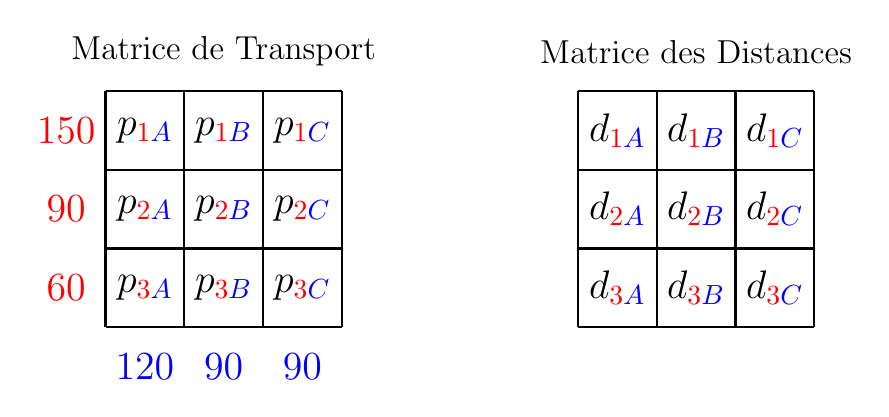
\begin{tikzpicture}
		\draw[step=1, thick] (0, 0) grid (3, 3);
		\node at (0.5, 0.5) {\Large $p_{{\color{red}3}{\color{blue}A}}$};
		\node at (1.5, 0.5) {\Large $p_{{\color{red}3}{\color{blue}B}}$};
		\node at (2.5, 0.5) {\Large $p_{{\color{red}3}{\color{blue}C}}$};
		\node at (0.5, 1.5) {\Large $p_{{\color{red}2}{\color{blue}A}}$};
		\node at (1.5, 1.5) {\Large $p_{{\color{red}2}{\color{blue}B}}$};
		\node at (2.5, 1.5) {\Large $p_{{\color{red}2}{\color{blue}C}}$};
		\node at (0.5, 2.5) {\Large $p_{{\color{red}1}{\color{blue}A}}$};
		\node at (1.5, 2.5) {\Large $p_{{\color{red}1}{\color{blue}B}}$};
		\node at (2.5, 2.5) {\Large $p_{{\color{red}1}{\color{blue}C}}$};
		
		\node at (1.5, 3.5) {\large Matrice de Transport};
		\node[blue] at (0.5, -0.5) {\Large 120};
		\node[blue] at (1.5, -0.5) {\Large 90};
		\node[blue] at (2.5, -0.5) {\Large 90};
		\node[red] at (-0.5, 0.5) {\Large 60};
		\node[red] at (-0.5, 1.5) {\Large 90};
		\node[red] at (-0.5, 2.5) {\Large 150};
		
		\node at (7.5, 3.5) {\large Matrice des Distances};
		\draw[step=1, thick] (6, 0) grid (9, 3);
		\node at (6.5, 0.5) {\Large $d_{{\color{red}3}{\color{blue}A}}$};
		\node at (7.5, 0.5) {\Large $d_{{\color{red}3}{\color{blue}B}}$};
		\node at (8.5, 0.5) {\Large $d_{{\color{red}3}{\color{blue}C}}$};
		\node at (6.5, 1.5) {\Large $d_{{\color{red}2}{\color{blue}A}}$};
		\node at (7.5, 1.5) {\Large $d_{{\color{red}2}{\color{blue}B}}$};
		\node at (8.5, 1.5) {\Large $d_{{\color{red}2}{\color{blue}C}}$};
		\node at (6.5, 2.5) {\Large $d_{{\color{red}1}{\color{blue}A}}$};
		\node at (7.5, 2.5) {\Large $d_{{\color{red}1}{\color{blue}B}}$};
		\node at (8.5, 2.5) {\Large $d_{{\color{red}1}{\color{blue}C}}$};
	\end{tikzpicture}
\end{center}

\paragraph{Cas discret}
En notant $D$ notre matrice des distances, on obtient la formulation suivante dans le cas discret :
$$ \min_P \langle P, D \rangle = \sum_i \sum_j p_{ij} d_{ij} $$
\vspace{-4mm}
$$ \text{s.t.} \quad \left\{ \begin{array}{ll}
\forall i & \sum_j p_{ij} = \mu_i \\
\forall j & \sum_i p_{ij} = \nu_j
\end{array} \right. $$

\paragraph{Cas continue}
Dans le cas continue on introduit l'ensemble des probabilités conjointes suivant :
$$ \Pi(\mu, \nu) = \left\{ P \in \mathcal{P}(\Omega \times \Omega)~|~\forall A, B \in \Omega, \, P(A \times \Omega) = \mu(A), \, P(\Omega \times B) = \nu(B) \right\} $$
Cet ensemble traduit les conditions du cas discret dans le cas continue. On reprend notre fonction de coût $c$ définie dans le problème de Monge. La formulation de Kantorovich devient le problème de minimisation suivant :
$$ \inf_{P \in \Pi(\mu, \nu)} \E_P \left[ c(X, Y) \right] = \int \int c(x, y) P(dx, dy) $$

\subs{Distance de Wasserstein}

Ce problème d'optimisation permet de définir une distance entre les mesures de probabilités.

\DEF{
	Étant donnée un espace de probabilité $\Omega$, une fonction de coût $c : \Omega \times \Omega \rightarrow \R$ et deux mesures de probabilités $\mu$ et $\nu$ dans $\mathcal{P}(\Omega)$, la \textbf{p-distance de Wasserstein} entre $\mu$ et $\nu$ est définie par :
	$$ W_p(\mu, \nu) = \left( \inf_{P \in \Pi(\mu, \nu)} \int \int c(x, y)^p P(dx, dy) \right)^{1 / p} $$
	\vspace{-3mm}
}

Cette distance peut permettre de calculer des barycentres entres des distributions de probabilité beaucoup plus naturels que des barycentres obtenus avec la norme $l_2$. La figure suivante nous montre la différence entre une interpolation (barycentre de deux distributions) obtenue via la distance de Wasserstein et une interpolation linéaire.

\begin{center}
	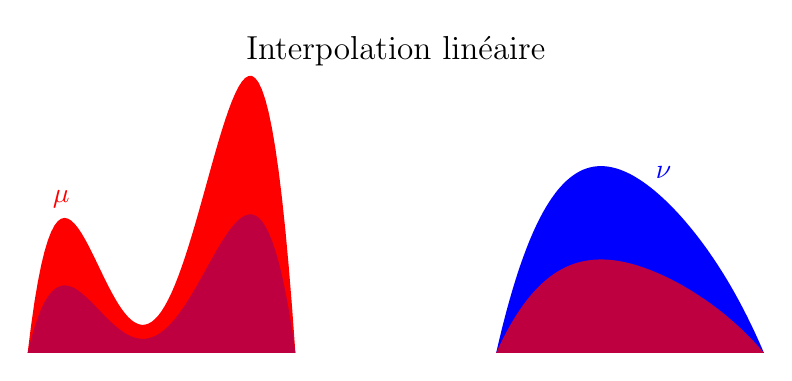
\begin{tikzpicture}[scale=0.85]
		\node at (5.5, 4.5) {\large Interpolation linéaire};
		\node[red] at (0.5, 2.3) {$\mu$};
		\node[blue] at (9.5, 2.7) {$\nu$};
		\fill[red] (0.000, 0.000) -- (0.050, 0.403) -- (0.100, 0.752) -- (0.150, 1.051) -- (0.200, 1.302) -- (0.250, 1.509) -- (0.300, 1.676) -- (0.350, 1.806) -- (0.400, 1.902) -- (0.450, 1.967) -- (0.500, 2.004) -- (0.550, 2.016) -- (0.600, 2.006) -- (0.650, 1.976) -- (0.700, 1.929) -- (0.750, 1.868) -- (0.800, 1.794) -- (0.850, 1.710) -- (0.900, 1.618) -- (0.950, 1.521) -- (1.000, 1.419) -- (1.050, 1.315) -- (1.100, 1.211) -- (1.150, 1.108) -- (1.200, 1.008) -- (1.250, 0.912) -- (1.300, 0.822) -- (1.350, 0.738) -- (1.400, 0.662) -- (1.450, 0.595) -- (1.500, 0.537) -- (1.550, 0.490) -- (1.600, 0.455) -- (1.650, 0.431) -- (1.700, 0.419) -- (1.750, 0.420) -- (1.800, 0.435) -- (1.850, 0.462) -- (1.900, 0.503) -- (1.950, 0.556) -- (2.000, 0.623) -- (2.050, 0.703) -- (2.100, 0.796) -- (2.150, 0.900) -- (2.200, 1.017) -- (2.250, 1.144) -- (2.300, 1.281) -- (2.350, 1.428) -- (2.400, 1.584) -- (2.450, 1.746) -- (2.500, 1.915) -- (2.550, 2.089) -- (2.600, 2.267) -- (2.650, 2.447) -- (2.700, 2.627) -- (2.750, 2.807) -- (2.800, 2.984) -- (2.850, 3.156) -- (2.900, 3.321) -- (2.950, 3.478) -- (3.000, 3.624) -- (3.050, 3.757) -- (3.100, 3.874) -- (3.150, 3.973) -- (3.200, 4.052) -- (3.250, 4.107) -- (3.300, 4.136) -- (3.350, 4.137) -- (3.400, 4.105) -- (3.450, 4.038) -- (3.500, 3.933) -- (3.550, 3.787) -- (3.600, 3.595) -- (3.650, 3.355) -- (3.700, 3.063) -- (3.750, 2.715) -- (3.800, 2.307) -- (3.850, 1.836) -- (3.900, 1.297) -- (3.950, 0.686) -- (4.000, 0.000);
		\fill[blue] (7.000, 0.000) -- (7.050, 0.215) -- (7.100, 0.418) -- (7.150, 0.611) -- (7.200, 0.792) -- (7.250, 0.964) -- (7.300, 1.126) -- (7.350, 1.278) -- (7.400, 1.421) -- (7.450, 1.555) -- (7.500, 1.681) -- (7.550, 1.798) -- (7.600, 1.907) -- (7.650, 2.008) -- (7.700, 2.102) -- (7.750, 2.188) -- (7.800, 2.268) -- (7.850, 2.341) -- (7.900, 2.408) -- (7.950, 2.468) -- (8.000, 2.522) -- (8.050, 2.571) -- (8.100, 2.614) -- (8.150, 2.652) -- (8.200, 2.685) -- (8.250, 2.713) -- (8.300, 2.737) -- (8.350, 2.755) -- (8.400, 2.770) -- (8.450, 2.781) -- (8.500, 2.787) -- (8.550, 2.790) -- (8.600, 2.790) -- (8.650, 2.785) -- (8.700, 2.778) -- (8.750, 2.767) -- (8.800, 2.754) -- (8.850, 2.737) -- (8.900, 2.718) -- (8.950, 2.696) -- (9.000, 2.672) -- (9.050, 2.645) -- (9.100, 2.615) -- (9.150, 2.584) -- (9.200, 2.550) -- (9.250, 2.514) -- (9.300, 2.476) -- (9.350, 2.436) -- (9.400, 2.394) -- (9.450, 2.350) -- (9.500, 2.305) -- (9.550, 2.257) -- (9.600, 2.208) -- (9.650, 2.157) -- (9.700, 2.104) -- (9.750, 2.050) -- (9.800, 1.993) -- (9.850, 1.935) -- (9.900, 1.875) -- (9.950, 1.814) -- (10.000, 1.750) -- (10.050, 1.685) -- (10.100, 1.618) -- (10.150, 1.549) -- (10.200, 1.477) -- (10.250, 1.404) -- (10.300, 1.329) -- (10.350, 1.251) -- (10.400, 1.172) -- (10.450, 1.090) -- (10.500, 1.005) -- (10.550, 0.918) -- (10.600, 0.828) -- (10.650, 0.736) -- (10.700, 0.640) -- (10.750, 0.542) -- (10.800, 0.440) -- (10.850, 0.336) -- (10.900, 0.227) -- (10.950, 0.116) -- (11.000, 0.000);
		\fill[purple] (0.000, 0.000) -- (0.050, 0.202) -- (0.100, 0.376) -- (0.150, 0.525) -- (0.200, 0.651) -- (0.250, 0.754) -- (0.300, 0.838) -- (0.350, 0.903) -- (0.400, 0.951) -- (0.450, 0.983) -- (0.500, 1.002) -- (0.550, 1.008) -- (0.600, 1.003) -- (0.650, 0.988) -- (0.700, 0.965) -- (0.750, 0.934) -- (0.800, 0.897) -- (0.850, 0.855) -- (0.900, 0.809) -- (0.950, 0.760) -- (1.000, 0.710) -- (1.050, 0.658) -- (1.100, 0.606) -- (1.150, 0.554) -- (1.200, 0.504) -- (1.250, 0.456) -- (1.300, 0.411) -- (1.350, 0.369) -- (1.400, 0.331) -- (1.450, 0.297) -- (1.500, 0.269) -- (1.550, 0.245) -- (1.600, 0.227) -- (1.650, 0.215) -- (1.700, 0.210) -- (1.750, 0.210) -- (1.800, 0.217) -- (1.850, 0.231) -- (1.900, 0.251) -- (1.950, 0.278) -- (2.000, 0.312) -- (2.050, 0.352) -- (2.100, 0.398) -- (2.150, 0.450) -- (2.200, 0.508) -- (2.250, 0.572) -- (2.300, 0.641) -- (2.350, 0.714) -- (2.400, 0.792) -- (2.450, 0.873) -- (2.500, 0.958) -- (2.550, 1.045) -- (2.600, 1.133) -- (2.650, 1.223) -- (2.700, 1.314) -- (2.750, 1.403) -- (2.800, 1.492) -- (2.850, 1.578) -- (2.900, 1.661) -- (2.950, 1.739) -- (3.000, 1.812) -- (3.050, 1.878) -- (3.100, 1.937) -- (3.150, 1.987) -- (3.200, 2.026) -- (3.250, 2.054) -- (3.300, 2.068) -- (3.350, 2.068) -- (3.400, 2.052) -- (3.450, 2.019) -- (3.500, 1.967) -- (3.550, 1.893) -- (3.600, 1.797) -- (3.650, 1.677) -- (3.700, 1.531) -- (3.750, 1.357) -- (3.800, 1.154) -- (3.850, 0.918) -- (3.900, 0.648) -- (3.950, 0.343) -- (4.000, 0.000);
		\fill[purple] (7.000, 0.000) -- (7.050, 0.107) -- (7.100, 0.209) -- (7.150, 0.305) -- (7.200, 0.396) -- (7.250, 0.482) -- (7.300, 0.563) -- (7.350, 0.639) -- (7.400, 0.711) -- (7.450, 0.778) -- (7.500, 0.840) -- (7.550, 0.899) -- (7.600, 0.953) -- (7.650, 1.004) -- (7.700, 1.051) -- (7.750, 1.094) -- (7.800, 1.134) -- (7.850, 1.171) -- (7.900, 1.204) -- (7.950, 1.234) -- (8.000, 1.261) -- (8.050, 1.286) -- (8.100, 1.307) -- (8.150, 1.326) -- (8.200, 1.343) -- (8.250, 1.357) -- (8.300, 1.368) -- (8.350, 1.378) -- (8.400, 1.385) -- (8.450, 1.390) -- (8.500, 1.394) -- (8.550, 1.395) -- (8.600, 1.395) -- (8.650, 1.393) -- (8.700, 1.389) -- (8.750, 1.384) -- (8.800, 1.377) -- (8.850, 1.369) -- (8.900, 1.359) -- (8.950, 1.348) -- (9.000, 1.336) -- (9.050, 1.322) -- (9.100, 1.308) -- (9.150, 1.292) -- (9.200, 1.275) -- (9.250, 1.257) -- (9.300, 1.238) -- (9.350, 1.218) -- (9.400, 1.197) -- (9.450, 1.175) -- (9.500, 1.152) -- (9.550, 1.129) -- (9.600, 1.104) -- (9.650, 1.078) -- (9.700, 1.052) -- (9.750, 1.025) -- (9.800, 0.997) -- (9.850, 0.968) -- (9.900, 0.938) -- (9.950, 0.907) -- (10.000, 0.875) -- (10.050, 0.842) -- (10.100, 0.809) -- (10.150, 0.774) -- (10.200, 0.739) -- (10.250, 0.702) -- (10.300, 0.664) -- (10.350, 0.626) -- (10.400, 0.586) -- (10.450, 0.545) -- (10.500, 0.502) -- (10.550, 0.459) -- (10.600, 0.414) -- (10.650, 0.368) -- (10.700, 0.320) -- (10.750, 0.271) -- (10.800, 0.220) -- (10.850, 0.168) -- (10.900, 0.114) -- (10.950, 0.058) -- (11.000, 0.000);
	\end{tikzpicture}
	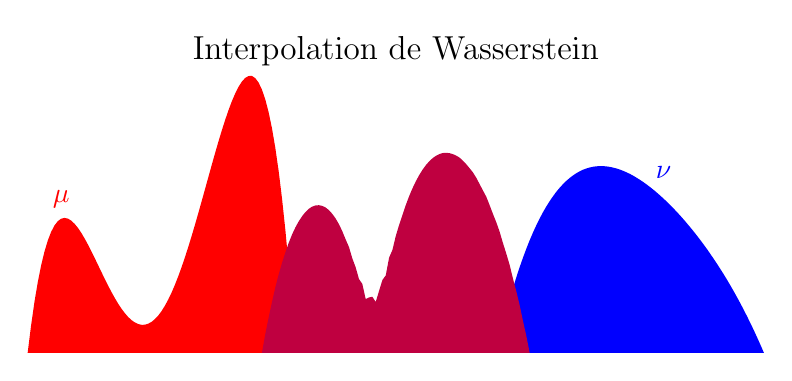
\begin{tikzpicture}[scale=0.85]
		\node at (5.5, 4.5) {\large Interpolation de Wasserstein};
		\node[red] at (0.5, 2.3) {$\mu$};
		\node[blue] at (9.5, 2.7) {$\nu$};
		\fill[red] (0.000, 0.000) -- (0.050, 0.403) -- (0.100, 0.752) -- (0.150, 1.051) -- (0.200, 1.302) -- (0.250, 1.509) -- (0.300, 1.676) -- (0.350, 1.806) -- (0.400, 1.902) -- (0.450, 1.967) -- (0.500, 2.004) -- (0.550, 2.016) -- (0.600, 2.006) -- (0.650, 1.976) -- (0.700, 1.929) -- (0.750, 1.868) -- (0.800, 1.794) -- (0.850, 1.710) -- (0.900, 1.618) -- (0.950, 1.521) -- (1.000, 1.419) -- (1.050, 1.315) -- (1.100, 1.211) -- (1.150, 1.108) -- (1.200, 1.008) -- (1.250, 0.912) -- (1.300, 0.822) -- (1.350, 0.738) -- (1.400, 0.662) -- (1.450, 0.595) -- (1.500, 0.537) -- (1.550, 0.490) -- (1.600, 0.455) -- (1.650, 0.431) -- (1.700, 0.419) -- (1.750, 0.420) -- (1.800, 0.435) -- (1.850, 0.462) -- (1.900, 0.503) -- (1.950, 0.556) -- (2.000, 0.623) -- (2.050, 0.703) -- (2.100, 0.796) -- (2.150, 0.900) -- (2.200, 1.017) -- (2.250, 1.144) -- (2.300, 1.281) -- (2.350, 1.428) -- (2.400, 1.584) -- (2.450, 1.746) -- (2.500, 1.915) -- (2.550, 2.089) -- (2.600, 2.267) -- (2.650, 2.447) -- (2.700, 2.627) -- (2.750, 2.807) -- (2.800, 2.984) -- (2.850, 3.156) -- (2.900, 3.321) -- (2.950, 3.478) -- (3.000, 3.624) -- (3.050, 3.757) -- (3.100, 3.874) -- (3.150, 3.973) -- (3.200, 4.052) -- (3.250, 4.107) -- (3.300, 4.136) -- (3.350, 4.137) -- (3.400, 4.105) -- (3.450, 4.038) -- (3.500, 3.933) -- (3.550, 3.787) -- (3.600, 3.595) -- (3.650, 3.355) -- (3.700, 3.063) -- (3.750, 2.715) -- (3.800, 2.307) -- (3.850, 1.836) -- (3.900, 1.297) -- (3.950, 0.686) -- (4.000, 0.000);
		\fill[blue] (7.000, 0.000) -- (7.050, 0.215) -- (7.100, 0.418) -- (7.150, 0.611) -- (7.200, 0.792) -- (7.250, 0.964) -- (7.300, 1.126) -- (7.350, 1.278) -- (7.400, 1.421) -- (7.450, 1.555) -- (7.500, 1.681) -- (7.550, 1.798) -- (7.600, 1.907) -- (7.650, 2.008) -- (7.700, 2.102) -- (7.750, 2.188) -- (7.800, 2.268) -- (7.850, 2.341) -- (7.900, 2.408) -- (7.950, 2.468) -- (8.000, 2.522) -- (8.050, 2.571) -- (8.100, 2.614) -- (8.150, 2.652) -- (8.200, 2.685) -- (8.250, 2.713) -- (8.300, 2.737) -- (8.350, 2.755) -- (8.400, 2.770) -- (8.450, 2.781) -- (8.500, 2.787) -- (8.550, 2.790) -- (8.600, 2.790) -- (8.650, 2.785) -- (8.700, 2.778) -- (8.750, 2.767) -- (8.800, 2.754) -- (8.850, 2.737) -- (8.900, 2.718) -- (8.950, 2.696) -- (9.000, 2.672) -- (9.050, 2.645) -- (9.100, 2.615) -- (9.150, 2.584) -- (9.200, 2.550) -- (9.250, 2.514) -- (9.300, 2.476) -- (9.350, 2.436) -- (9.400, 2.394) -- (9.450, 2.350) -- (9.500, 2.305) -- (9.550, 2.257) -- (9.600, 2.208) -- (9.650, 2.157) -- (9.700, 2.104) -- (9.750, 2.050) -- (9.800, 1.993) -- (9.850, 1.935) -- (9.900, 1.875) -- (9.950, 1.814) -- (10.000, 1.750) -- (10.050, 1.685) -- (10.100, 1.618) -- (10.150, 1.549) -- (10.200, 1.477) -- (10.250, 1.404) -- (10.300, 1.329) -- (10.350, 1.251) -- (10.400, 1.172) -- (10.450, 1.090) -- (10.500, 1.005) -- (10.550, 0.918) -- (10.600, 0.828) -- (10.650, 0.736) -- (10.700, 0.640) -- (10.750, 0.542) -- (10.800, 0.440) -- (10.850, 0.336) -- (10.900, 0.227) -- (10.950, 0.116) -- (11.000, 0.000);
		\fill[purple] (3.500, 0.000) -- (3.550, 0.279) -- (3.600, 0.526) -- (3.650, 0.758) -- (3.700, 0.977) -- (3.750, 1.171) -- (3.800, 1.343) -- (3.850, 1.500) -- (3.900, 1.643) -- (3.950, 1.768) -- (4.000, 1.874) -- (4.050, 1.965) -- (4.100, 2.041) -- (4.150, 2.103) -- (4.200, 2.151) -- (4.250, 2.184) -- (4.300, 2.202) -- (4.350, 2.206) -- (4.400, 2.196) -- (4.450, 2.172) -- (4.500, 2.133) -- (4.550, 2.078) -- (4.600, 2.009) -- (4.650, 1.923) -- (4.700, 1.819) -- (4.750, 1.696) -- (4.800, 1.582) -- (4.850, 1.413) -- (4.900, 1.279) -- (4.950, 1.102) -- (5.000, 1.030) -- (5.050, 0.804) -- (5.100, 0.828) -- (5.150, 0.838) -- (5.200, 0.760) -- (5.250, 0.925) -- (5.300, 1.088) -- (5.350, 1.157) -- (5.400, 1.422) -- (5.450, 1.538) -- (5.500, 1.746) -- (5.550, 1.912) -- (5.600, 2.060) -- (5.650, 2.209) -- (5.700, 2.342) -- (5.750, 2.459) -- (5.800, 2.564) -- (5.850, 2.656) -- (5.900, 2.736) -- (5.950, 2.805) -- (6.000, 2.862) -- (6.050, 2.908) -- (6.100, 2.944) -- (6.150, 2.969) -- (6.200, 2.985) -- (6.250, 2.989) -- (6.300, 2.984) -- (6.350, 2.970) -- (6.400, 2.948) -- (6.450, 2.919) -- (6.500, 2.874) -- (6.550, 2.821) -- (6.600, 2.761) -- (6.650, 2.700) -- (6.700, 2.620) -- (6.750, 2.525) -- (6.800, 2.430) -- (6.850, 2.336) -- (6.900, 2.211) -- (6.950, 2.080) -- (7.000, 1.955) -- (7.050, 1.814) -- (7.100, 1.644) -- (7.150, 1.485) -- (7.200, 1.317) -- (7.250, 1.113) -- (7.300, 0.921) -- (7.350, 0.715) -- (7.400, 0.477) -- (7.450, 0.255) -- (7.500, 0.000);
	\end{tikzpicture}
\end{center}

On rappelle que le calcul du barycentre $\mu$ des des $N$ distributions $\nu_i$ associé aux poids $\lambda_i$ revient au problème de minimisation suivant :
$$ \min_{\mu \in \mathcal{P}(\Omega)} \sum_{i=1}^N \lambda_i W_p^p(\mu, \nu_i) $$
Et voici maintenant ce que donne des barycentres avec 4 distributions :
\begin{center}
	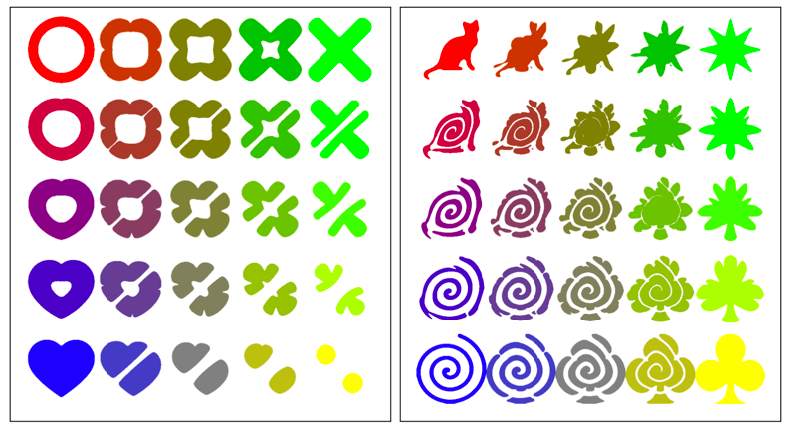
\includegraphics[scale=0.4]{wasserstein_bar.png}
\end{center}

\sect{Comment calculer le transport optimal ?}

\subs{Dual}

Pour les calculs on revient vers les espaces discrets. Nos mesures de probabilité sont des sommes de diracs :
$$ \mu = \sum_{i=1}^n a_i \delta_{x_i} \qquad \nu = \sum_{j =1}^m b_j \delta_{y_j} $$
Notre fonction de coût est une matrice $D \in \R_+^{n \times m}$ tel que $D_{ij} = d(x_i, y_j)^p$. Notre distribution conjointe $P$ est aussi une matrice de $\R_+^{n \times m}$ qui doit vérifier certaines contraintes pouvant se représenter de manière matricielle. L'ensemble dans lequel se trouve $P$ est le suivant :
$$ U(a, b) = \left\{ P \in \R_+^{n \times m}~|~P \mathbbm{1}_m = a, \, P^\trans \mathbbm{1}_n = b \right\} $$

\DEF{
	La définition de la distance de Wasserstein dans un espace discret est la suivante :
	$$ W_p^p(\mu, \nu) = \min_{P \in U(a, b)} \langle P, D \rangle $$
	\vspace{-6mm}
}

\paragraph{Dual} On s'intéresse maintenant au problème dual. On introduit le lagrangien :
$$ L(P, \alpha, \beta) = \langle P, D \rangle + \alpha^\trans (a - P \mathbbm{1}_m) + \beta^\trans (b - P^\trans \mathbbm{1}_n) $$
La fonction objective du dual est :
$$ g(\alpha, \beta) = \min_{P \geqslant 0} L(P, \alpha, \beta) = \min_{P \geqslant 0} \alpha^\trans a + \beta^\trans b + \langle P, D - \alpha \mathbbm{1}_m^\trans - \mathbbm{1}_n \beta^\trans \rangle $$
Si la matrice $D - \alpha \mathbbm{1}_m^\trans - \mathbbm{1}_n \beta^\trans$ possède un coefficient négatif alors en faisant tendre le même coefficient de la matrice $P$ vers $+\infty$ on obtient pour minimum $-\infty$. En revanche si tous les coefficients sont positifs alors $\langle P, D - \alpha \mathbbm{1}_m^\trans - \mathbbm{1}_n \beta^\trans \rangle$ est positif et il suffit de prendre $P=0$ pour se retrouver avec une valeur nulle. On obtient alors :
$$ g(\alpha, \beta) = \left\{ \begin{array}{ll}
\alpha^\trans a + \beta^\trans b & \text{si } D - \alpha \mathbbm{1}_m^\trans - \mathbbm{1}_n \beta^\trans \geqslant 0 \\
-\infty & \text{sinon}
\end{array}\right. $$
Finalement le dual est la maximisation de cette fonction $g$.

\DEF{
	Le \textbf{dual} du transport optimal a la formulation suivante :
	$$ W_p^p(\mu, \nu) = \max_{\alpha \in \R^n, \, \beta \in \R^m \atop \alpha_i + \beta_j \leqslant D(x_i, y_j)^p} \alpha^\trans a + \beta^\trans b $$
	\vspace{-5mm}
}

Avec un solveur de flot de coût minimum on peut résoudre cette optimisation linéaire en temps $\mathcal{O}(n^3 \log (n))$. Mais la solution est instable. Comme illustré sur la figure ci-dessous. Si on change un peu notre distance $D$ ou si on modifie un peu nos mesures source et destination $\mu$ et $\nu$ la valeur de $P$ peut subir un changement brutal puisque $P$ est un sommet de notre simplex. Une solution consiste à faire une régularisation de notre problème pour se retrouver avec un ensemble $U_\alpha(a, b)$ strictement convexe. Cet ensemble est strictement inclus dans $U(a, b)$ et la solution optimale de ce nouveau problème ne sera plus optimal pour le problème initial mais sera tout de même correcte. Finalement la régularisation que l'on va voire permet aussi d'obtenir un algorithme de résolution itératif de moindre complexité.

\begin{center}
	\begin{tikzpicture}[scale=20, >={latex}]
		\clip (0.2, -0.01) rectangle (0.51, 0.2);
		\draw[blue, thick] (0.1420, 0.1407) -- (0.5970, -0.1407);
		\draw[black, ->, thick] (0.2038, 0.1216) -- (0.2507, 0.1975);
		\fill[brown!40] (0.4503, 0.1444) -- (0.2251, 0.1444) -- (0.3695, 0.0000) -- (0.4503, -0.0000);
		\fill[greenTikz!60] (0.3827, 0.0946) -- (0.3827, 0.1104) -- (0.3804, 0.1148) -- (0.3759, 0.1206) -- (0.3692, 0.1263) -- (0.3602, 0.1307) -- (0.3556, 0.1321) -- (0.3489, 0.1336) -- (0.3264, 0.1336) -- (0.3219, 0.1321) -- (0.3151, 0.1278) -- (0.3129, 0.1234) -- (0.3129, 0.1191) -- (0.3151, 0.1133) -- (0.3241, 0.1018) -- (0.3444, 0.0888) -- (0.3534, 0.0859) -- (0.3714, 0.0859) -- (0.3804, 0.0917);
		\node[blue] at (0.3444, 0.0888) {$\bullet$};
		\node[blue, below=2] at (0.3444, 0.0888) {$P_\alpha$};
		\node[greenTikz] at (0.3489, 0.1119) {$\bullet$};
		\node[red] at (0.3695, 0.0000) {$\bullet$};
		\node[red, above=2] at (0.3695, 0) {$P$};
		\node at (0.482, 0.08) {$U(a, b)$};
		\node at (0.413, 0.12) {$U_\alpha(a, b)$};
		\node at (0.213, 0.165) {$D$};
	\end{tikzpicture}
\end{center}

\subs{Régularisation}

La régularisation que l'on effectue consiste à maximiser l'entropie de probabilité conjointe $P$. On fait apparaître un nouveau paramètre $\gamma$ qui contrôle cette régularisation et on obtient la distance suivante :

\DEF{
	La \textbf{distance de Wasserstein régularisée} est définie de la manière suivante :
	$$ W_\gamma(\mu, \nu) = \min_{P \in U(a, b)} \langle P, D \rangle - \gamma H(P) $$
	\vspace{-5mm}
} 

\paragraph{Remarque}
On rappelle que l'on peut considérer deux variables aléatoires $X$ et $Y$ tel que $X \sim \mu$, $Y \sim \nu$ et $X, Y \sim P$. L'entropie de $P$ est maximale lorsque $X$ et $Y$ sont indépendants, c'est à dire lorsque $P = ab^\trans$ et l'entropie maximal est alors $H(\mu) + H(\nu)$. La régularisation donne donc une matrice avec des valeurs strictement positive plus réparties.

\begin{center}
	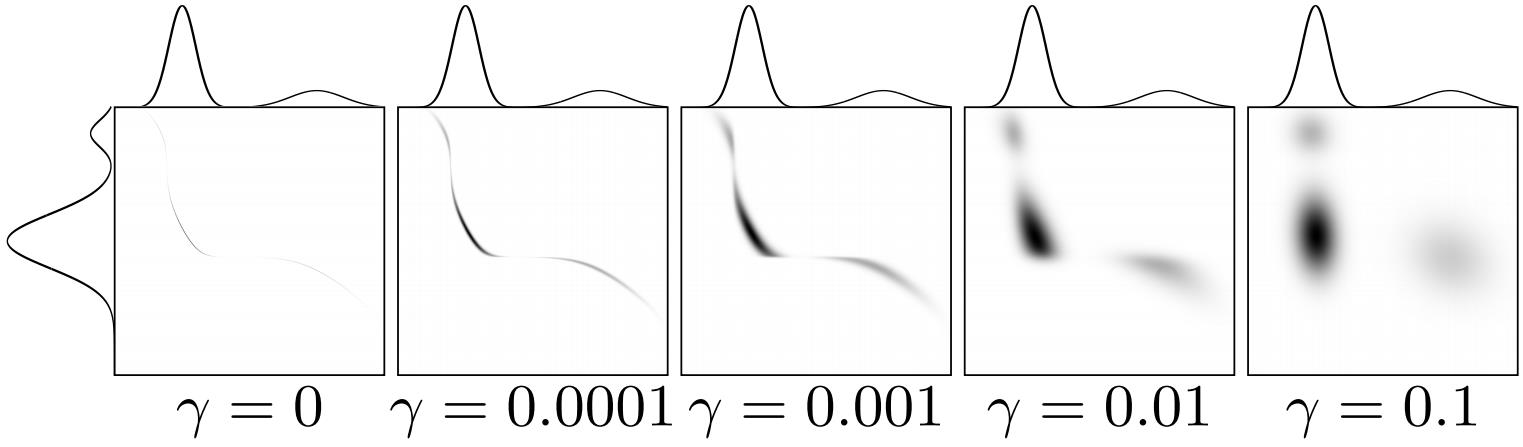
\includegraphics[scale=0.25]{reg_wass.png}
\end{center}

Par stricte convexité, il existe une unique matrice $P_\gamma$ qui minimise la distance :
$$ P_\gamma = \argmin_{P \in U(a, b)} \langle P, D \rangle - \gamma H(P) $$

\PROP{
	Il existe un unique couple de vecteurs $u$ et $v$ appartenant à $\R_+^n$ et $\R_+^m$ tel que :
	$$ P_\gamma = \text{diag}(u) K \text{diag}(v), \qquad K = e^{-D / \gamma} $$
	\vspace{-6mm}
}

\dem
On écrit le nouveau laplacien :
$$ L(P, \alpha, \beta) = \sum_{ij} \left( P_{ij} D_{ij} + \gamma P_{ij} \left( \log_2 P_{ij} - 1 \right) \right) + \alpha^\trans (a - P \mathbbm{1}_m) + \beta^\trans (b - P^\trans \mathbbm{1}_n) $$
On calcule alors la dérivée partielle par rapport à $P_{ij}$ :
$$ \dfrac{\partial L}{\partial P_{ij}} = M_{ij} + \gamma \log_2 P_{ij} - \alpha_i - \beta_j $$
Le dual est la maximisation du minimum du laplacien par rapport à $P$. Donc on doit avoir $P$ tel que la dérivée partielle est nulle :
$$ \dfrac{\partial L}{\partial P_{ij}} = 0 \Rightarrow P_{ij} = e^{\frac{\alpha_i}{\gamma}} e^{-\frac{D_{ij}}{\gamma}}  e^{\frac{\beta_j}{\gamma}} = u_i K_{ij} v_j $$
\findem

\paragraph{Sinkhorn}
On dispose alors d'une méthode itérative pour trouver cette matrice $P_\gamma$. On traduit la condition $P_\gamma \in U(a, b)$ :
$$ P_\gamma \in U(a, b) \Leftrightarrow \left\{ \begin{array}{lrr}
\text{diag}(u) K \text{diag}(v) \mathbbm{1}_m & = & a \\
\text{diag}(v) K^\trans \text{diag}(u) \mathbbm{1}_n & = & b
\end{array} \right. $$
$$ P_\gamma \in U(a, b) \Leftrightarrow \left\{ \begin{array}{lrr}
\text{diag}(u) K v & = & a \\
\text{diag}(v) K^\trans u & = & b
\end{array} \right. $$
On introduit alors $\odot$ le produit coefficient par coefficient :
$$ P_\gamma \in U(a, b) \Leftrightarrow \left\{ \begin{array}{lrr}
u \odot K v & = & a \\
v \odot K^\trans u & = & b
\end{array} \right. $$
$$ P_\gamma \in U(a, b) \Leftrightarrow \left\{ \begin{array}{lrc}
u & = & a \, / \, K v \\
v & = & b \, / \, K^\trans u
\end{array} \right. $$
L'algorithme de Sinkhorn est alors le suivant :\\
\begin{algorithm}[H]
	\caption{Sinkhorn}
	\Repeat{convergence de $u, v$}{
		$u \gets a \, / \, K v$ \;
		$v \gets b \, / \, K^\trans u$ \;
	}
\end{algorithm}

\paragraph{Complexité}
Il a été prouvé que l'algorithme converge en temps linéaire. De plus une étape de calcul se fait en $\mathcal{O}(nm)$ mais les calculs peuvent être parallélisés. Il est aussi possible d'utiliser des convolutions sur une grille pour obtenir une complexité en $\mathcal{O}(n \log n)$.

\paragraph{Dual}
On peut aussi relever la formulation du dual avec régularisation :
$$ W_\gamma(\mu, \nu) = \max_{\alpha, \beta} \alpha^\trans a + \beta^\trans b - \gamma \left( e^{\alpha / \gamma} \right)^\trans K \left( e^{\beta / \gamma} \right) $$

\paragraph{Lien avec la divergence KL}
En posant le noyau :
$$ K_\gamma(i, j) = \exp \left( - \dfrac{d_{i, j}}{\gamma} \right) $$
On obtient une reformulation de la régularisation entropique avec la divergence KL :
$$ W_\gamma(\mu, \nu) = \min_{P \in U(a, b)} \gamma KL(P | K_\gamma) $$

\sect{Optimal Transport and Machine Learning}

\subs{Compute the optimal transport of what?}

Since Sinkhorn can be parallelized, one can compute a large amount of Optimal
Transport distances: for instance look into a database for similarity based
retrieval, blablabla

\paragraph{Color histograms}

For image retrieval blablabla...

\paragraph{Cloud of word}

For similar documents retrieval blabla

\subs{Wassersteinization}

Introduce Wasserstein distance into optimizations problem.

We show that we can computationaly differentiate, and therefore we can deal
with it in a variety of optimization problem, including machine learning
related opt. problems. 

Somehow revisiting machine learning problems.

\paragraph{Averaging data}

histograms, distribution, images, experiments (repetition of same expriment,
MEG mesures, average over the experiments might be relevant)

\paragraph{Aggregating distributions}

From a very big dataset, split it in $J$ parts, learn the distribution (eg. w/
Bayesaian Learning) from each of the part in parralel (on $J$ machines):
the $J$ distributions should not be very different, but still the variance in
the data will cause some variation: the idea is to use Wasserstein averaging
to aggregate the distributions, and get a more meaningful one. Theoretic
guaranties! :D

Wasserstein posterior

%\subs{Semi-suppervised learning setting}

\paragraph{Semi-supervised learning setting}

Wasserstein propagation: smooth a graph $(V,E)$ where an histogram is associated
$\mu_v$ to each vertex $v$, with a susbset $S$ of the vertices that have a
fixed histogram (known data).

Solve the following optimization problem.

$$
    \underset{\substack{\mu_i \in \mathcal{P}\left(\Omega\right) \\ \text{for }i \in V\setminus S}}\min \sum_{(e_1, e_2) \in E} W_2^2\left(\mu_{e_1}, \mu_{e_2}\right)
$$

blabla

\paragraph{omg dictionnary learning what is this????????? :oooooo}

\subs{Wasserstein PCA, Geodesics and Inverse problem}

Since the space of distributions with the OT geometry has negative curvature,
we generalize the PCA (ie. projecting on one dimension spaces) into Generalized
Principal Geodesics. We then want to explain stuff out of what we found;
eg. affaire Bonneel vs nounours
